\documentclass[a4paper,12pt]{article}
\usepackage{graphicx}
\usepackage{hyperref}
\usepackage{array}

\title{User Guide - Online Test Monitoring System}
\date{} % This removes the date

\begin{document}

\maketitle

\tableofcontents
\newpage

\section{Introduction}
The \textbf{Online Test Monitoring System} is an AI-powered solution designed to monitor online exams by detecting fraud attempts using the YOLOv11 detection model. The application analyzes faces captured by the webcam in real time and identifies spoofing attempts using the \textbf{CelebA\_Spoof} dataset.

\begin{figure}[h!]
    \centering
    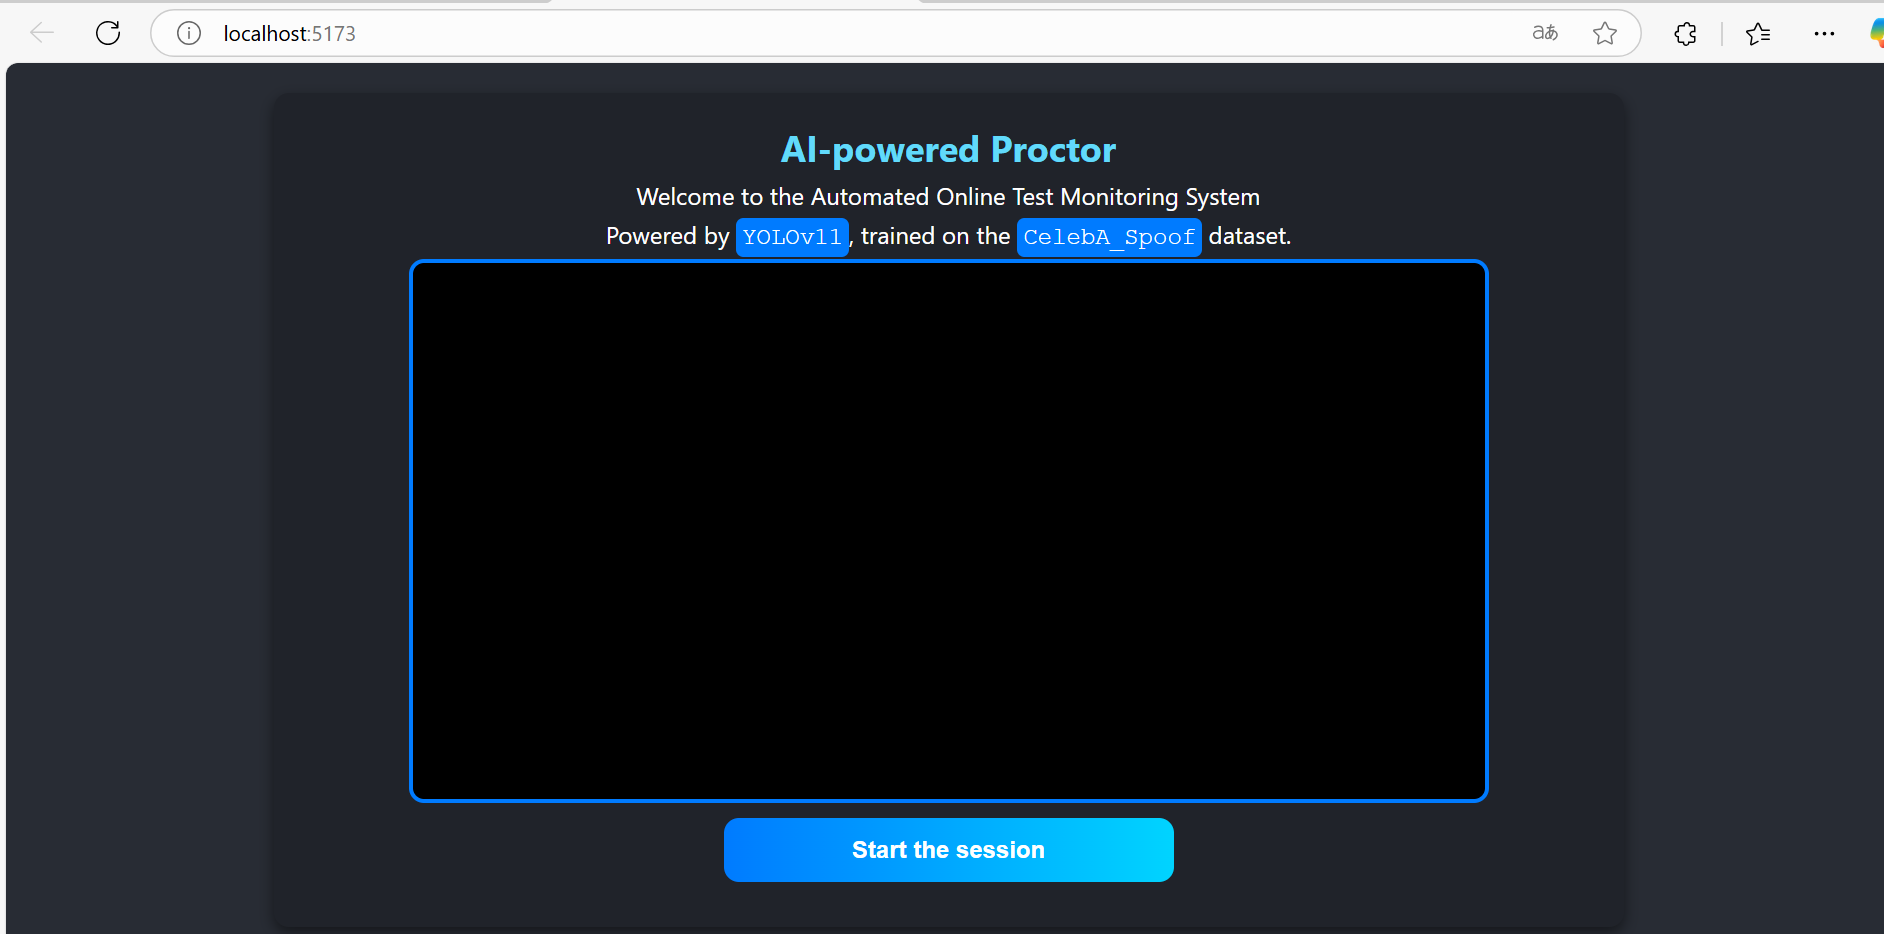
\includegraphics[width=0.8\textwidth]{IMG/accueil.png}
    \caption{Welcome screen of the Online Test Monitoring System}
    \label{fig:welcome_screen}
\end{figure}

\section{System Requirements}
\subsection{Hardware}
\begin{itemize}
    \item Computer with a functional webcam.
    \item Stable Internet connection.
    \item Compatible browsers: Google Chrome, Mozilla Firefox, Microsoft Edge (latest versions).
\end{itemize}

\subsection{Software}
\begin{itemize}
    \item Web-based application accessible via browser.
    \item No installation or backend required.
\end{itemize}

\section{Launching the Application}
\begin{enumerate}
    \item Open a compatible browser.
    \item Navigate to the application URL
    \item The main screen displays the \textbf{``Start the session''} button. 
\end{enumerate}

\begin{figure}[h!]
    \centering
    
\includegraphics[width=0.8\textwidth]{IMG/start_session_btn.png}
    \caption{Starting button}
    \label{fig:welcome_screen}
\end{figure}


\section{Starting a Monitoring Session}
\begin{enumerate}
    \item Click on \textbf{``Start the session''}.
    \item A form appears requesting the candidate's and sponsor's email addresses.
    \item Enter the required information and click \textbf{``Start the session''} again.
\end{enumerate}

\begin{figure}[h!]
    \centering
    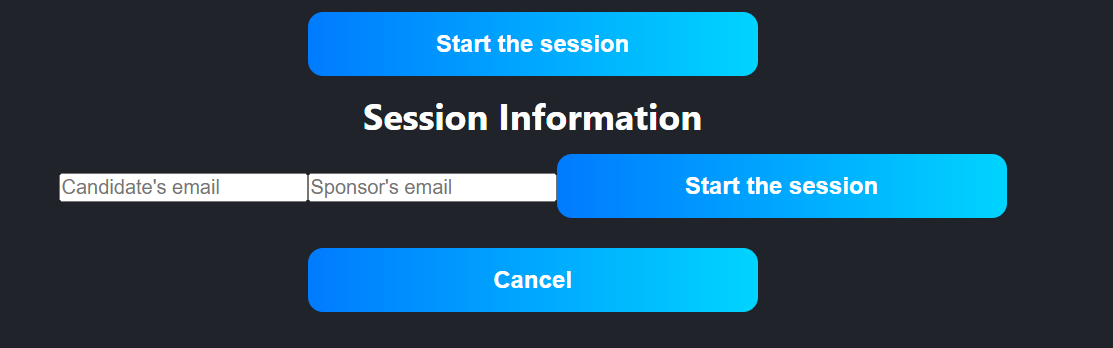
\includegraphics[width=0.8\textwidth]{IMG/email_registration.png}
    \caption{Welcome screen of the Online Test Monitoring System}
    \label{fig:welcome_screen}
\end{figure}

\begin{enumerate}
    \setcounter{enumi}{3}
    \item The application starts and activates the webcam for real-time monitoring.
    \item Face detection appears on the screen, indicating whether the user is real or suspicious.
\end{enumerate}

\begin{figure}[h!]
    \centering
    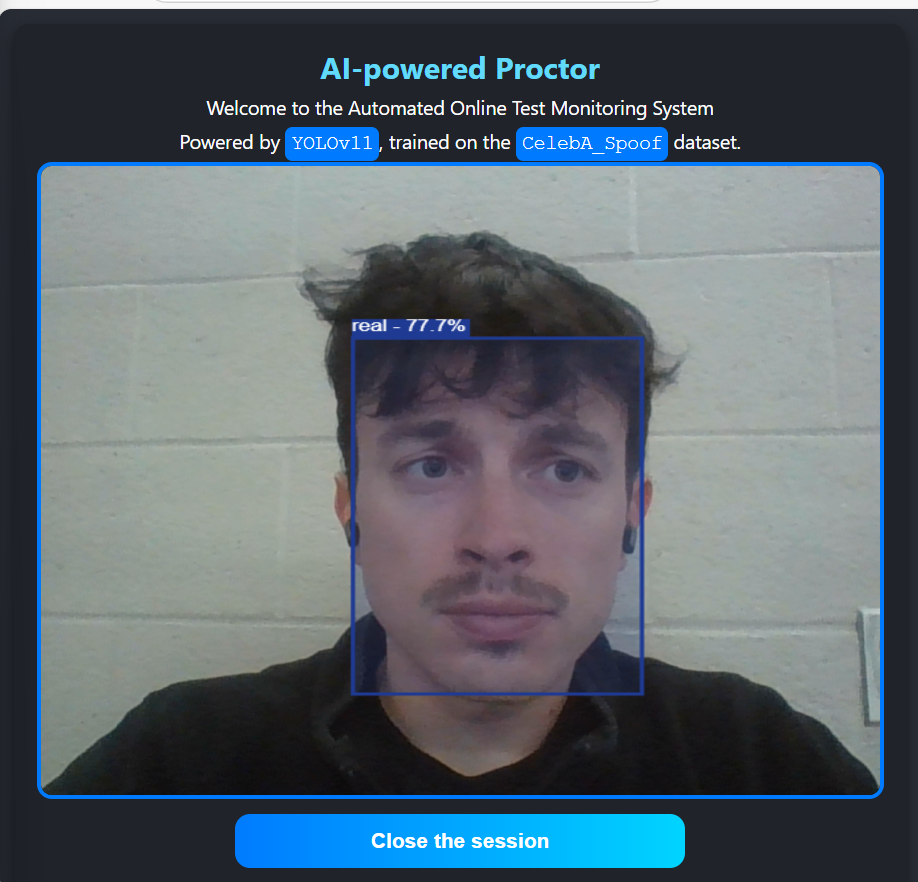
\includegraphics[width=0.8\textwidth]{IMG/session.png}
    \caption{Session running}
    \label{fig:welcome_screen}
\end{figure}

\section{Session Results Analysis}
\begin{itemize}
    \item The application displays a \textbf{fraud detection probability} as a percentage.
    \item Example:
    \begin{itemize}
        \item \textbf{Real - 54.3\%}: The user appears to be real with 54.3\% confidence (Displayed with a blue square around the face).
        \item \textbf{Spoof - 95.45\%}: High suspicion of fraud (Displayed with a red square around the face).
    \end{itemize}
    \item After the exam, a \textbf{session summary} is displayed.
\end{itemize}

\begin{figure}[h!]
    \centering
    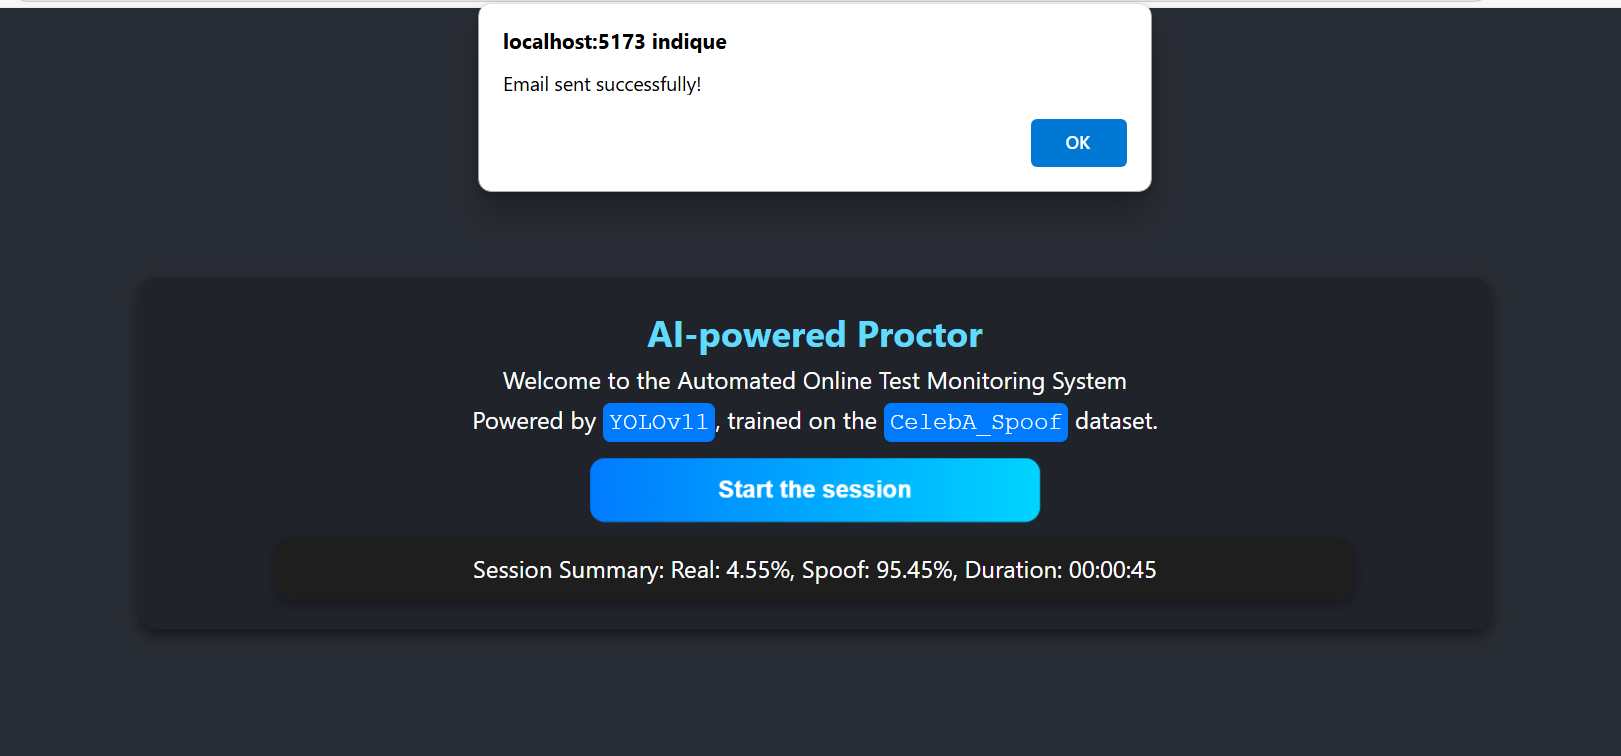
\includegraphics[width=0.8\textwidth]{IMG/session_end.png}
    \caption{Session summary}
    \label{fig:welcome_screen}
\end{figure}

\section{Sending the Session Report}
\begin{enumerate}
    \item After the exam ends, a summary email is sent.
    \item The user receives a confirmation message: \textbf{``Email sent successfully!''}.
\end{enumerate}

\begin{figure}[h!]
    \centering
    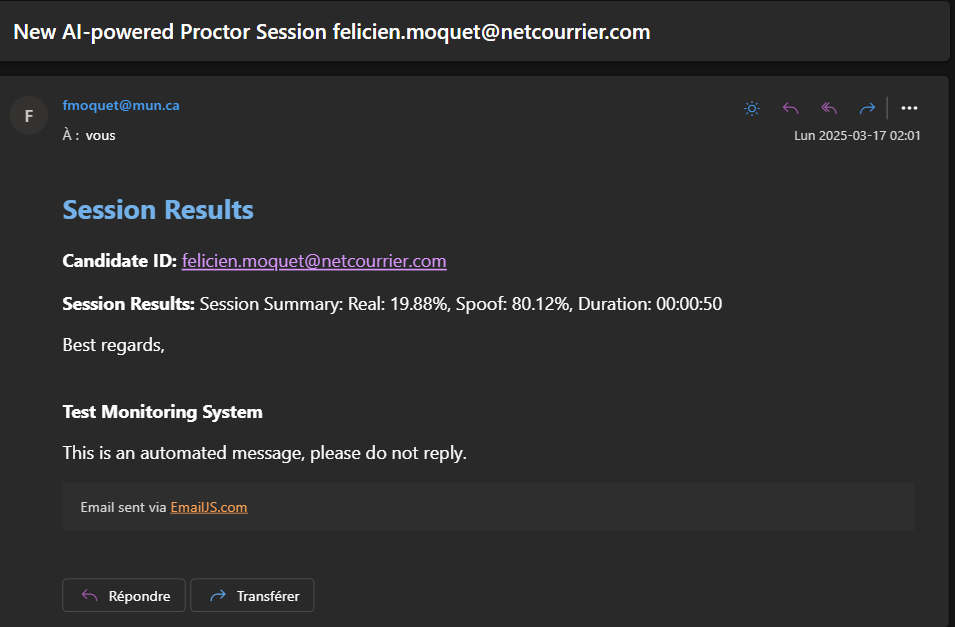
\includegraphics[width=0.8\textwidth]{IMG/email.png}
    \caption{email received}
    \label{fig:welcome_screen}
\end{figure}

\section{Important Notice}
The \textbf{Online Test Monitoring System} is based on artificial intelligence, which functions as a probabilistic tool. This means that while the system aims to detect fraudulent activities as accurately as possible, it does not guarantee 100\% accuracy. The results should not be used to take definitive actions against any individual without further human verification. The developers cannot ensure complete reliability of the detection process and are not responsible for any misclassification or potential errors produced by the system.

\section{Troubleshooting Common Issues}
\begin{tabular}{|p{6cm}|p{8cm}|}
    \hline
    \textbf{Issue} & \textbf{Solution} \\
    \hline
    Webcam not working & Check browser permissions. \\
    \hline
    The model does not detect the face properly & Ensure you are well-lit and facing the camera. \\
    \hline
    Application not responding & Refresh the page and restart the session. \\
    \hline
\end{tabular}

\section{Contact and Support}
For any questions or technical issues, please contact our support team via email: \textbf{support@proctoring-ai.com}.

\end{document}
